\subsection[Contexte social et écologique]{Une entreprise dans un contexte social et \\écologique}
\paragraph{Impact sur l'Environnement}
\begin{wrapfigure}[12]{o}{8cm}
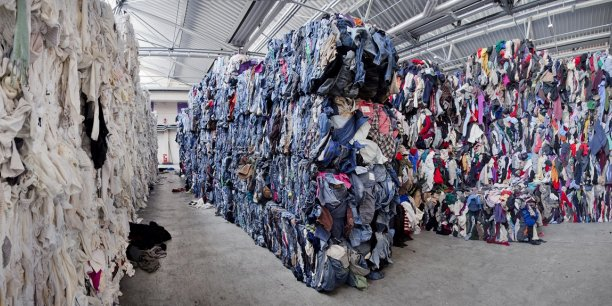
\includegraphics[width=8cm]{image/recyclage.jpg}
\end{wrapfigure}
L'industrie du textile est maintenant la deuxième industrie la plus polluante après la production pétro-chimique\footnote{www.commeuncamion.com/2018/09/02/pourquoi-la-mode-est-devenue-une-des-industries-les-plus-polluantes/}. Pourtant cette question est peu présente dans l'industrie du sur mesure. Il peut néanmoins servir d'argument commercial pour le sur-mesure de luxe qui produit souvent au Portugal. Sinon peux de clients s'intéresse à la provenance de leurs costumes. Une petite étude auprès de mes camarades ma appris qu'une magorité ne savais pas que leurs costumes venait de Thailande. Quel est sont impact par rapport à l'industrie du pret à porté. En premier lieu, un habit sur mesure sera en général garder plus longtemps qu'une pièce de la \textit{fast fashion}. Cependant les délais de livraison extrèment cours demandés obligent des trajets aériens intercontinentaux contrairement aux vetements ordinaires arrivant principalement par voie maritime.
\paragraph{Aspect sociologique}
Les entreprises française ont obligation de se renseigner sur leurs fournisseurs, c'est la Resposabilité Sociale des Entreprise (RSE)\footnote{www.e-rse.net/definitions/rse-definition/}. Nous pouvons néamoins nous demander dans quelle mesure les tailleurs s'intéresse réellement aux conditions de travail des employés du textil en Thailande. En effet il est courant d'avoir un atelier \textit{"de démonstration"} et une usine plus effective. Cependant j'ai pu durant mon stage visiter une usine (sans prendre de photo). Les conditions de travail sont correcte avec des locaux climatisés et des postes assis ergonomiques. Ces métiers recrutent autant de femme que d'homme qui sont payés également, ils sont en effet payé à la pièce. D'après notre employeur ce mode de payment est réclamé par les employés car celà leurs permettrait de prendre des jours chomés quand ils le souhaiteraient.
